\documentclass{beamer}
\usepackage[utf8]{inputenc}

\usetheme{Madrid}
\usecolortheme{default}
\usepackage{amsmath,amssymb,amsfonts,amsthm}
\usepackage{txfonts}
\usepackage{tkz-euclide}
\usepackage{listings}
\usepackage{adjustbox}
\usepackage{array}
\usepackage{tabularx}
\usepackage{gvv}
\usepackage{lmodern}
\usepackage{circuitikz}
\usepackage{tikz}
\usepackage{graphicx}
\usepackage{amsmath}
\usepackage{mathtools}
\setbeamertemplate{page number in head/foot}[totalframenumber]

\usepackage{tcolorbox}
\tcbuselibrary{minted,breakable,xparse,skins}



\definecolor{bg}{gray}{0.95}
\DeclareTCBListing{mintedbox}{O{}m!O{}}{%
  breakable=true,
  listing engine=minted,
  listing only,
  minted language=#2,
  minted style=default,
  minted options={%
    linenos,
    gobble=0,
    breaklines=true,
    breakafter=,,
    fontsize=\small,
    numbersep=8pt,
    #1},
  boxsep=0pt,
  left skip=0pt,
  right skip=0pt,
  left=25pt,
  right=0pt,
  top=3pt,
  bottom=3pt,
  arc=5pt,
  leftrule=0pt,
  rightrule=0pt,
  bottomrule=2pt,
  toprule=2pt,
  colback=bg,
  colframe=orange!70,
  enhanced,
  overlay={%
    \begin{tcbclipinterior}
    \fill[orange!20!white] (frame.south west) rectangle ([xshift=20pt]frame.north west);
    \end{tcbclipinterior}},
  #3,
}
\lstset{
    language=C,
    basicstyle=\ttfamily\small,
    keywordstyle=\color{blue},
    stringstyle=\color{orange},
    commentstyle=\color{green!60!black},
    numbers=left,
    numberstyle=\tiny\color{gray},
    breaklines=true,
    showstringspaces=false,
}


\title 
{7.2.18}



\author 
{Pratik R-AI25BTECH11023}



\begin{document}


\frame{\titlepage}
%------------------------------------
\begin{frame}{Question}
Find the equation of the circle passing through $(0, 0)$ and making intercepts $a$ and $b$ on the coordinate axes.
\end{frame}
\begin{frame}{Solution}
Let:
\begin{align}
\vec{x_1} = \myvec{0 \\ 0},\ \vec{x_2} = \myvec{a \\ 0},\ \vec{x_3} = \myvec{0 \\ b}
\end{align}
\end{frame}
\begin{frame}{Solution}
We use the general matrix form of a circle:
\begin{align}
\myvec{2x_1 & 2x_2 & 2x_3\\
1 & 1 & 1}^T \myvec{\vec{u} \\ f} = - \myvec{\norm{x_1}^2 \\ \norm{x_2}^2 \\ \norm{x_3}^2}
\end{align}

Substituting the values:

\begin{align}
\myvec{
0 & 0 & 1 \\
2a & 0 & 1 \\
0 & 2b & 1
}
\myvec{
u_1 \\
u_2 \\
f
}
=
- \myvec{
0 \\
a^2 \\
b^2
}
\end{align}
\end{frame}
\begin{frame}{Solution}
Using augmented matrix and

applying $R_1\leftrightarrow R_2$

and $R_2\leftrightarrow R_3$

\begin{align}
\myvec{
2a & 0 & 1 &\vrule &-a^2 \\ 
0 & 2b & 1 &\vrule &-b^2\\
0 & 0 & 1 &\vrule &0 
} \xleftrightarrow{R_1=R_1 - R_3}\xleftrightarrow{R_2=R_2 - R_3}
\myvec{
2a & 0 & 0 &\vrule &-a^2 \\ 
0 & 2b & 0 &\vrule &-b^2\\
0 & 0 & 1 &\vrule &0 
}
\end{align}
\end{frame}
\begin{frame}{Solution}
we get
\begin{align}
\vec{u} = \myvec{ -\frac{a}{2} \\ -\frac{b}{2} }, \quad f = 0
\end{align}

So the equation of the circle becomes:


\begin{align}
x^2 + y^2 + ax + by = 0
\end{align}
\end{frame}
\begin{frame}{plot}
\centering
    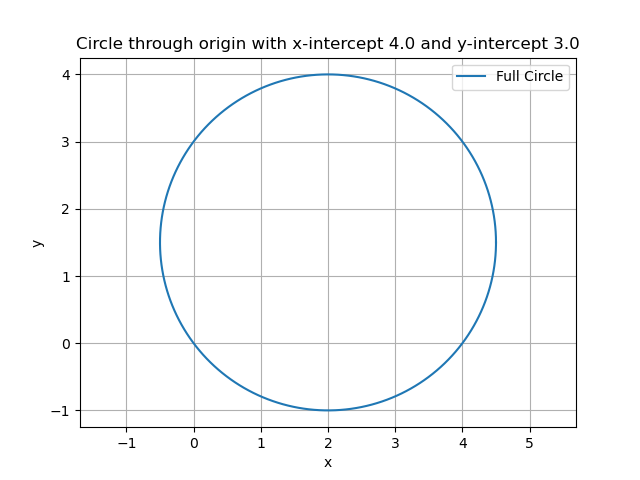
\includegraphics[width=\columnwidth, height=0.8\textheight, keepaspectratio]{../figs/fig.png}     
\end{frame}

\end{document}